\documentclass[tikz,border=2pt]{standalone}
\usepackage{tikz}
\usetikzlibrary{positioning}
\begin{document}
% Namikawa--Ueno type: IV^*-I_l-t
% Target MRNC type: IV^*-I_l-t
% Adapted from Tim Dokchitser picture: I_{{\it n}}\e({\it m})IV^*
% Parameter substitution: n -> l, m -> t
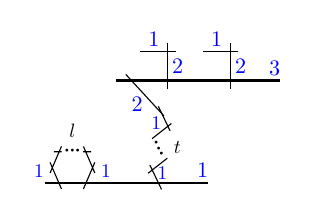
\begin{tikzpicture}[xscale=0.57,yscale=0.62]
\draw[thick,shorten >=2] (-0.09,0)--(3.67,0) node[inner sep=2pt,blue,above left,scale=0.8] {1};
\draw[scale=0.8] (0,0) ++(0.05,0.3) node[anchor=east,blue,scale=0.7] {1} ++(0.3,-0.45)--++(115:0.75)++(295:0.15)++(245:0.15)--++(65:0.75)++(245:0.15)++(180:0.15)--++(0:0.22) ++(0:0.15) node{$\cdot$} ++(0:0.15) node{$\cdot$} node[above=0.1,anchor=south,scale=0.7]{$l$}++(0:0.15) node{$\cdot$} ++(0:0.15) --++(0:0.22)++(180:0.15)++(115:0.15)--++(295:0.75)++(115:0.15)++(65:0.15)--++(245:0.75)++(0.3,0.45) node[anchor=west,blue,scale=0.7] {1};\draw (2.44,0) 
    ++(0.07,-0.13)--++(-0.26,0.5)++(0.12,-0.19)  
    ++(0,0.02)
      node[blue,scale=0.7,inner sep=1,anchor=west]{1}
    ++(0,-0.02)
    ++(-0.16,0.02)--++(0.43,0.31)++(-0.13,0.07)  
    node{$\cdot$} ++(-0.06,0.12) node{$\cdot$}
    ++(-0.06,0.12) node{$\cdot$}++(0.17,-0.1)    node[auto,inner sep=5,scale=0.7,anchor=west]{$t$}
    ++(-0.26,0.19)--++(0.43,0.31)++(-0.18,0.04)   
    ++(0,-0.04)
      node[blue,scale=0.7,inner sep=1,anchor=east]{1}
    ++(0,0.04)
    ++(0.18,-0.04)++(-0.03,-0.15)--++(-0.26,0.5);
\draw[shorten <=-3pt, shorten >=-3pt] (2.44,3/2)--node[inner sep=2pt,scale=0.8,blue,below left=-1pt and -1pt] {2} (1.84,21/10);
\draw[thick,shorten >=2] (1.5,21/10)--(5.27,21/10) node[inner sep=2pt,blue,above left,scale=0.8] {3};
\draw[shorten <=-3pt, shorten >=-3pt] (2.64,21/10)--node[inner sep=2pt,scale=0.8,blue,right] {2} (2.64,27/10);
\draw[shorten <=-3pt] (2.64,27/10)--node[inner sep=2pt,scale=0.8,blue,above] {1} (2.04,27/10);
\draw[shorten <=-3pt, shorten >=-3pt] (4.04,21/10)--node[inner sep=2pt,scale=0.8,blue,right] {2} (4.04,27/10);
\draw[shorten <=-3pt] (4.04,27/10)--node[inner sep=2pt,scale=0.8,blue,above] {1} (3.44,27/10);
\end{tikzpicture}
\end{document}
